\newpage
\section{Methodik und Vorgehen} \label{sec:Methodik und Vorgehen}

Das methodische Vorgehen dieser Masterthesis basiert auf der \ac{DSR}-Methodologie, die auf die systematische Entwicklung und Evaluierung von Artefakten zur Lösung relevanter Probleme abzielt \parencite[S. 78]{hevner_DesignScienceInformationsystemsresearch_2004}. Die Literaturrecherche folgt den von \textcite{page_PRISMA2020Statementupdatedguidelinereportingsystematicreviews_2021} entwickelten \ac{PRISMA} 2020 Richtlinien.

Ziel des \ac{DSR} ist es, wissenschaftlich fundiertes Gestaltungswissen zu schaffen und praxisrelevante Lösungen zu validieren \parencite[S. 83]{hevner_DesignScienceInformationsystemsresearch_2004}. Die Leitlinien fordern die zielgerichtete Entwicklung und verständliche Beschreibung eines innovativen Artefakts, dessen Nutzen belegt sowie gründlich evaluiert und klar kommuniziert wird \parencite[S. 82]{hevner_DesignScienceInformationsystemsresearch_2004}.

Dieses Vorgehen eignet sich besonders zur Entwicklung eines quantenresistenten \ac{SSI}-Prototyps, da es eine methodisch fundierte Brücke zwischen Theorie und Praxis schlägt und den Nutzen für reale Anwendungsfelder sichert.

Das methodische Vorgehen dieser Arbeit basiert auf dem Drei-Zyklen-Modell nach \textcite[S. 88]{hevner_ThreeCycleViewDesignScienceResearch_2007} (\autoref{fig:Design Science Research Cycles}). Die Verknüpfung von Relevance Cycle (KRITIS-Anforderungen), Rigor Cycle (systematische Literaturrecherche nach \ac{PRISMA} 2020) und Design Cycle (iterative Prototyp-Entwicklung) sichert eine fundierte und praxisnahe Umsetzung.

\begin{figure}[H]
    \centering
    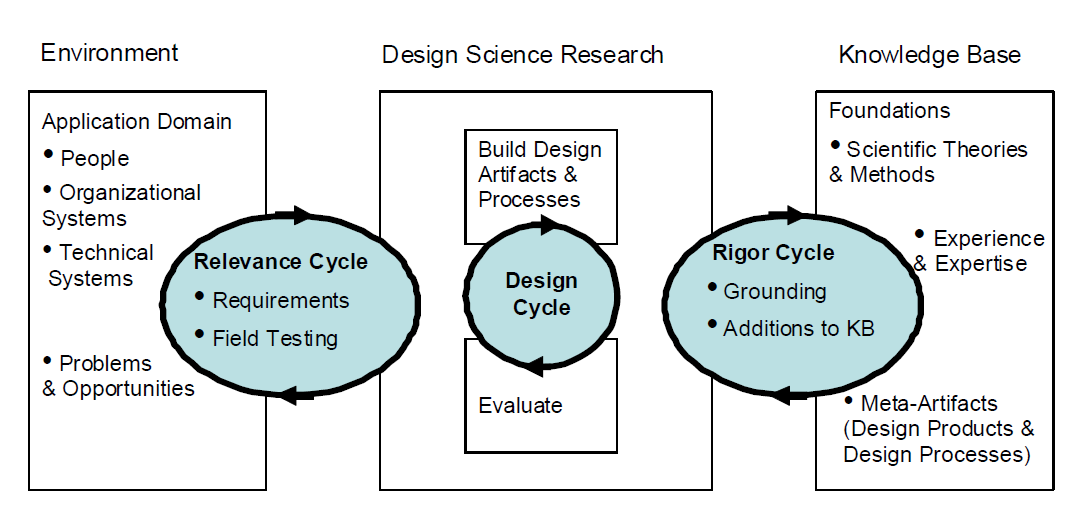
\includegraphics[width=\linewidth]{3-cycle.png}
    \caption{Design Science Research Cycles}
    \begin{flushleft}
    \textit{Anmerkung.} Aus \textcite[S. 88]{hevner_ThreeCycleViewDesignScienceResearch_2007}.
    \end{flushleft}
    \label{fig:Design Science Research Cycles}
\end{figure}

Für die Umsetzung des \ac{DSR} wird das sechsstufige Prozessmodell nach \textcite[S. 54]{peffers_DesignScienceResearchmethodologyinformationsystemsresearch_2007} (\autoref{fig:DSRM Process Model}) adaptiert und sichert eine systematische Strukturierung des Forschungsvorhabens.

Durch iterative Rückkopplung insbesondere zu Zieldefinition und Design/Entwicklung kann das Artefakt laufend anhand von Evaluationen und neuen Anforderungen optimiert werden. Die Praxisnähe ist durch die Orientierung an realen Use Cases und \ac{KRITIS}-Anforderungen gewährleistet.

\begin{figure}[H]
    \centering
    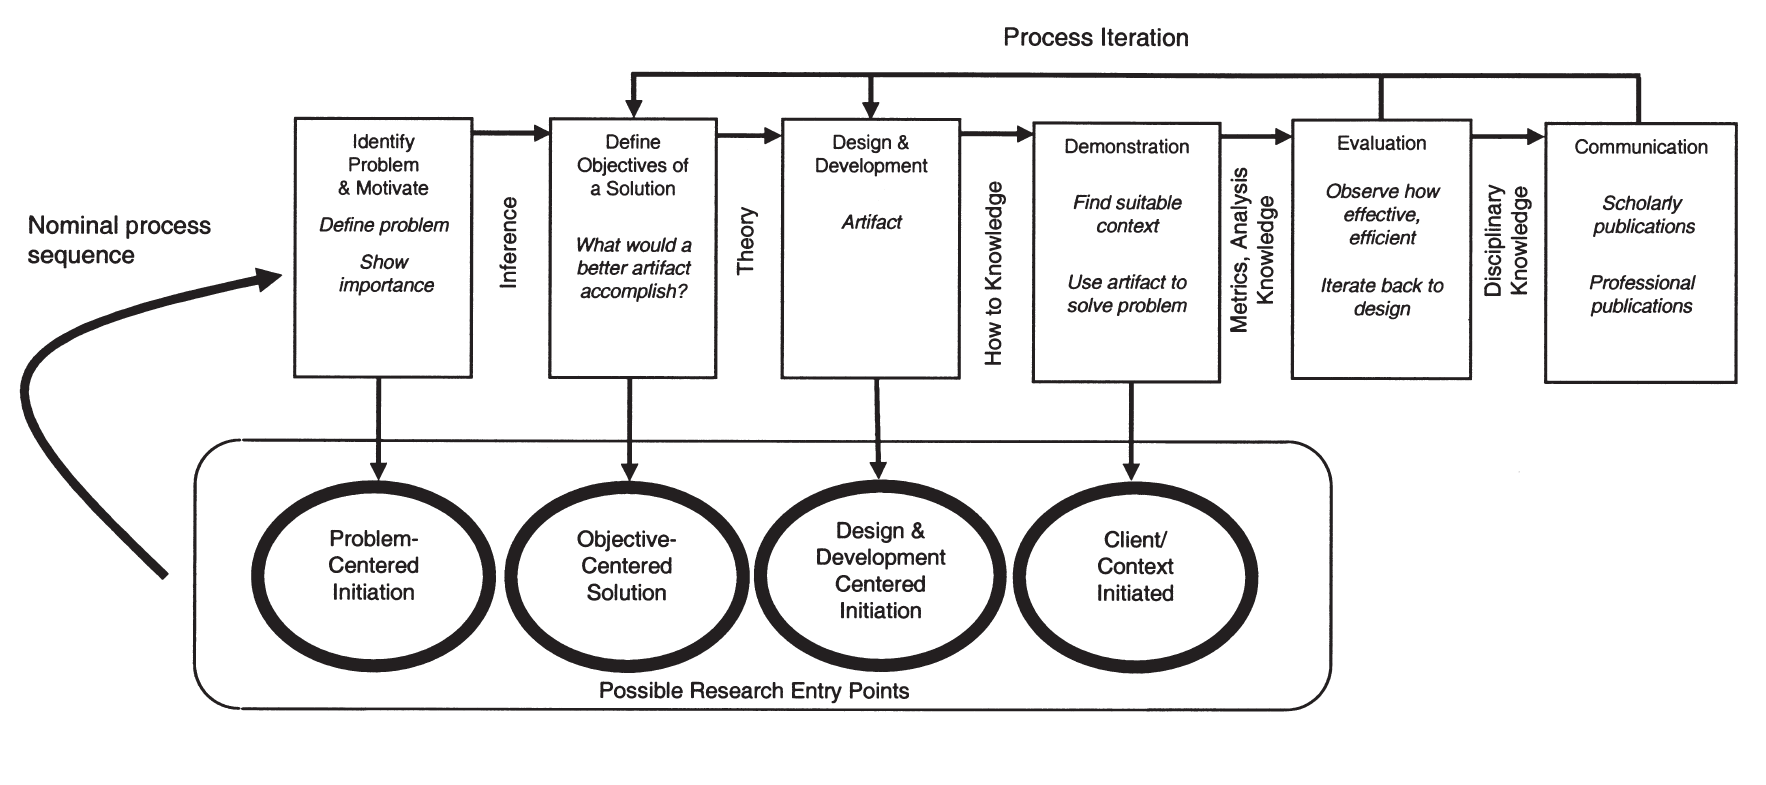
\includegraphics[width=\linewidth]{DSRM Process Model.png}
    \caption{DSRM Process Model}
    \begin{flushleft}
    \textit{Anmerkung.} Aus \textcite[S. 54]{peffers_DesignScienceResearchmethodologyinformationsystemsresearch_2007}.
    \end{flushleft}
    \label{fig:DSRM Process Model}
\end{figure}

\pagebreak

Die konkrete Umsetzung der sechs \ac{DSR}-Phasen zeigt \autoref{tab:dsr_phasen}.

\begin{longtable}{L{3.5cm}L{11cm}}
    \caption{Konkrete Anwendung des DSRM Process Modells}
    \label{tab:dsr_phasen} \\
    \toprule
    \textbf{Phase} & \textbf{Beschreibung} \\
    \midrule
    \endfirsthead
    \multicolumn{2}{l}{\textit{Tabelle \thetable\ (Fortsetzung)}} \\
    \toprule
    \textbf{Phase} & \textbf{Beschreibung} \\
    \midrule
    \endhead
    \midrule
    \multicolumn{2}{r}{\textit{Fortsetzung auf nächster Seite}} \\
    \endfoot
    \bottomrule
    \multicolumn{2}{p{\linewidth}}{\textit{Anmerkung.} Eigene Darstellung auf Basis von \textcite[S. 54]{peffers_DesignScienceResearchmethodologyinformationsystemsresearch_2007} mit Inhalten des vorliegenden Exposes und \textcite[S. 1]{venable_FEDSFrameworkEvaluationDesignScienceResearch_2016}.} \\
    \endlastfoot
    Phase 1: \newline Problemidentifikation und Motivation &
    Identifikation der drohenden Quantenbedrohung für bestehende \ac{SSI}-Systeme für \ac{KRITIS} als zentrale Herausforderung. \\
    \midrule
    Phase 2: \newline Zieldefinition &
    Konkretisierung der vier Forschungsfragen zu Systemarchitektur, Algorithmenauswahl, Performance und kryptografischer Agilität als Rahmengebung des Lösungsansatzes. \\
    \midrule
    Phase 3: \newline Design und Entwicklung &
    Festlegung des Technologie-Stacks, Architekturentscheidungen, die Auswahl und Integration der \ac{PQC}-Algorithmen sowie die Definition geeigneter Schnittstellen und Datenflüsse. Darüber hinaus werden die spezifischen Compliance-Anforderungen für \ac{KRITIS} in das Systemdesign integriert. Die Implementierung innerhalb der Laborumgebung erfolgt modular, um kryptografische Agilität zu gewährleisten und zukünftige Algorithmus-Updates ohne Systemunterbrechung zu ermöglichen. Sie umfasst die (Weiter-)Entwicklung zentraler Systemkomponenten und Mechanismen für zentrale Aktivitäten des Identity Management Lifecycles. \\
    \midrule
    Phase 4: \newline Demonstration &
    Verifizierung der grundsätzlichen Funktionsfähigkeit des entwickelten Prototyps innerhalb der Laborumgebung anhand voridentifizierter Use Cases, die auf dem Identity Management Lifecycle aufbauen und ausgewählte Szenarien des \ac{KRITIS}-Bereichs darstellen. \\
    \midrule
    Phase 5: \newline Evaluation &
    Multidimensionale Anwendung des von \textcite{venable_FEDSFrameworkEvaluationDesignScienceResearch_2016} entwickelten \ac{FEDS}-Frameworks, welches eine systematische Bewertungsstrategie für \ac{DSR}-Artefakte bereitstellt. Die Evaluation gliedert sich nach \textcite[S. 1]{venable_FEDSFrameworkEvaluationDesignScienceResearch_2016} in formative und summative Komponenten, wobei sowohl künstliche als auch naturalistische Evaluationsparadigmen zum Einsatz kommen. \\
    \midrule
    Phase 6: \newline Kommunikation &
    Weitergabe der Forschungsergebnisse. Im Rahmen dieser Masterarbeit erfolgt dies in einem ausgewählten Rahmen, wobei sowohl wissenschaftliche als auch praxisorientierte Zielgruppen berücksichtigt werden. Die Ergebnisse zur Integration von \ac{PQC} in \ac{SSI}-Systeme werden in Form von Gestaltungsprinzipien zusammengefasst, um Anhaltspunkte für zukünftige Entwicklungen in diesem Bereich zu bieten. \\
\end{longtable}